\documentclass[12pt,a4paper]{article}
\usepackage{enumerate} %item
\usepackage{CJKutf8} %chinese
\usepackage{graphicx} %insert figure
\usepackage{amsmath}
\graphicspath{ {E:\類神經\HW1\hw1.png} }

\title{Introduction to Neural Networks \\ Homework \#1}
\author{機械所 \\張元睿 \\N16054629}
\date{\today}


\begin{document}

	\begin{CJK}{UTF8}{bsmi}
	\maketitle
	\newpage
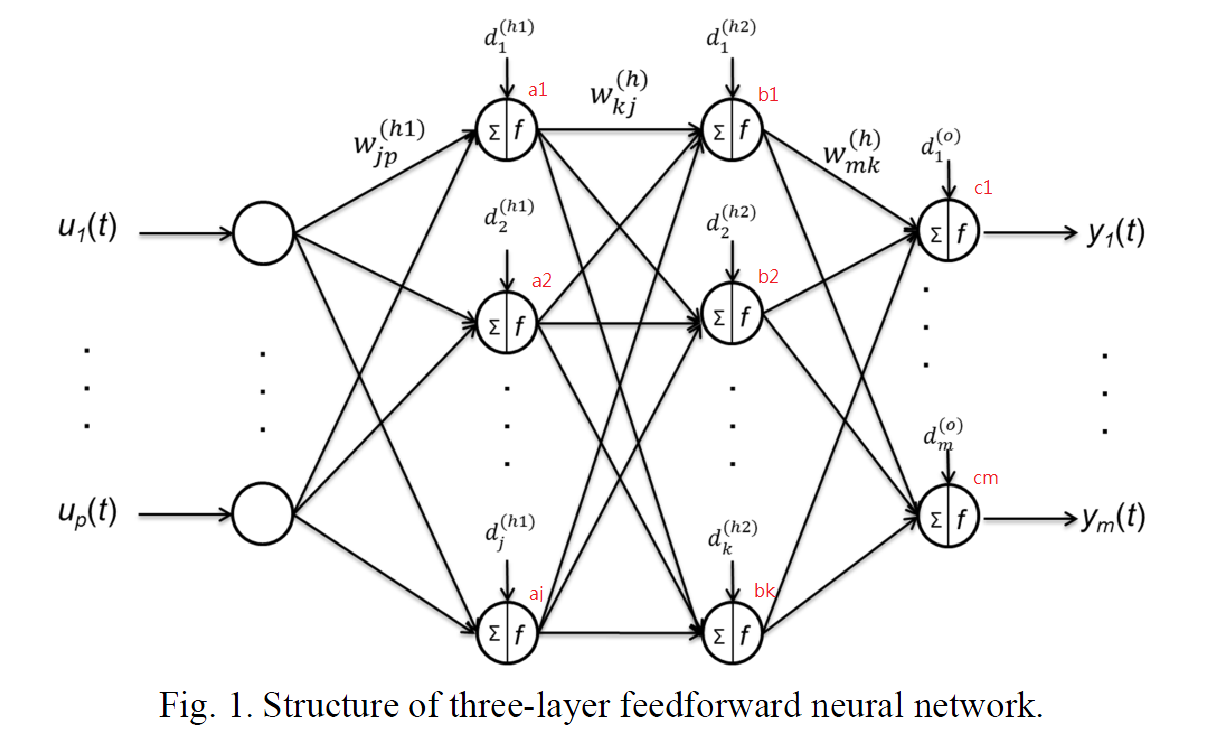
\includegraphics[scale=0.5]{hw1}

\begin{enumerate}
	\vspace{1cm}
	\item Forward path:
\vspace{0.5cm}
\\	
	$a_j=\sum\limits_{\alpha=1 \sim j,\  \beta=1 \sim p}
w_{\alpha\beta}^{(h1)} \times u_\beta(t)+d_\alpha^{(h1)} $
\vspace{0.5cm}
\\
	$Y_{a_j}=sigmoid(a_j)=\frac{1}{1+ e^{-a_j}}$
\vspace{0.5cm}
\\
	$b_k=\sum\limits_{\alpha=1 \sim k,\  \beta=1 \sim j}
w_{\alpha\beta}^{(h2)} \times Y_{a_\beta}+d_\alpha^{(h2)} $
\vspace{0.5cm}
\\
	$Y_{b_k}=\tanh(b_k)=\frac{e^{b_k}-e^{-b_k}}{e^{b_k}+e^{-b_k}}$
\vspace{0.5cm}
\\
	$y_m(t)=c_m=\sum\limits_{\alpha=1 \sim m,\  \beta=1 \sim k}
	w_{\alpha\beta}^{(h3)} \times y_{b_\beta}+d_\alpha^{(o)} $
\\[0.5cm]
\noindent\rule{\textwidth}{1pt}
\\[0.5cm]
$E_m(t)=\frac{1}{2}e_m^2(t)
\\[0.5cm]
e_m(t)=d_m(t)-y_m(t)
$
\newpage
\item Backward propagation
\begin{enumerate}
	\item Update rule for the weights of the output neurons:
\vspace{0.5cm}
\\
$
	\begin{aligned}
	w_{mk}^{(h_3)}(t+1) & =w_{mk}^{(h_3)}(t)+\Delta w_{mk}(t)
\\[0.5cm]
	& =	w_{mk}^{(h_3)}(t)-\eta\frac{\partial E_m(t)}{\partial w_{mk}^{(h_3)}(t)}
\\[0.5cm]
	& = w_{mk}^{(h_3)}(t)-\eta\frac{\partial E_m(t)}{\partial e_{m}(t)}
	\frac{\partial e_{m}(t)}{\partial y_m(t)}
	\frac{\partial y_m(t)}{\partial c_{m}(t)}
	\frac{\partial c_m(t)}{\partial w_{mk}^{(h_3)}(t)}
\\[0.5cm]
	& = w_{mk}^{(h_3)}(t)-\eta(d_m(t)-y_m(t))(-1)(1)(Y_{b_k}(t))
\\[0.5cm]
	& = w_{mk}^{(h_3)}(t)+\eta(d_m(t)-y_m(t))(Y_{b_k}(t))	
	\end{aligned}
$
	\item Update rule for the biases of the output neurons:
\vspace{0.5cm}
\\
$
\begin{aligned}
d_{m}^{(o)}(t+1) & =d_{m}^{(o)}(t)+\Delta d_{m}(t)
\\[0.5cm]
& =d_{m}^{(o)}(t)-\eta\frac{\partial E_m(t)}{\partial d_{m}^{(o)}(t)}
\\[0.5cm]
& =d_{m}^{(o)}(t)-\eta\frac{\partial E_m(t)}{\partial e_{j}(t)}
\frac{\partial e_{m}(t)}{\partial y_m(t)}
\frac{\partial y_m(t)}{\partial c_{m}(t)}
\frac{\partial c_m(t)}{\partial d_{m}^{(o)}(t)}
\\[0.5cm]
& =d_{m}^{(o)}(t)-\eta(d_m(t)-y_m(t))(-1)(1)(1)
\\[0.5cm]
& =d_{m}^{(o)}(t)+\eta(d_m(t)-y_m(t))
\end{aligned}
$
\newpage

	\item Update rule for the weights of the second hidden neurons:
\vspace{0.5cm}
\\
$
\begin{aligned}
w_{kj}^{(h_2)}(t+1) & =w_{kj}^{(h_2)}(t)+\Delta w_{kj}(t)
\\[0.5cm]
& =	w_{kj}^{(h_2)}(t)-\eta\frac{\partial E_m(t)}{\partial w_{kj}^{(h_2)}(t)}
\\[0.5cm]
& = w_{kj}^{(h_2)}(t)-\eta\frac{\partial E_m(t)}{\partial e_{m}(t)}
\frac{\partial e_{m}(t)}{\partial y_m(t)}
\frac{\partial y_m(t)}{\partial c_{m}(t)}
\frac{\partial c_m(t)}{\partial Y_{b_k}(t)}
\frac{\partial Y_{b_k}(t)}{\partial b_k(t)}
\frac{\partial b_k(t)}{\partial w_{kj}^{(h_2)}(t)}
\\[0.5cm]
& = w_{kj}^{(h_2)}(t)-\eta\sum_m(d_m(t)-y_m(t))(-1)(1)(w_{mk}^{(h_3)}(t))[1-\tanh^2(b_k(t))]
\\[0.5cm]
&\ \hspace{11cm}
(Y_{a_j}(t))
\\[0.5cm]
& = w_{kj}^{(h_2)}(t)+\eta\sum_m(d_m(t)-y_m(t))(w_{mk}^{(h_3)}(t))[1-\tanh^2(b_k(t))](Y_{a_j}(t))
\end{aligned}
$

	\item Update rule for the biases of the second hidden neurons:
\vspace{0.5cm}
\\
$
\begin{aligned}
d_{k}^{(h_2)}(t+1) & =d_{k}^{(h_2)}(t)+\Delta d_{k}(t)
\\[0.5cm]
& =d_{k}^{(h_2)}(t)-\eta\frac{\partial E_m(t)}{\partial d_{k}^{(h_2)}(t)}
\\[0.5cm]
& =d_{k}^{(h_2)}(t)-\eta\frac{\partial E_m(t)}{\partial e_{j}(t)}
\frac{\partial e_{m}(t)}{\partial y_m(t)}
\frac{\partial y_m(t)}{\partial c_{m}(t)}
\frac{\partial c_m(t)}{\partial Y_{b_k}(t)}
\frac{\partial Y_{b_k}(t)}{\partial b_k(t)}
\frac{\partial b_k(t)}{\partial d_j^{(h_1)}(t)}
\\[0.5cm]
& =d_{k}^{(h_2)}(t)-\eta\sum_m(d_m(t)-y_m(t))(-1)(1)(w_{mk}^{(h_3)}(t))[1-\tanh^2(b_k(t))](1)
\\[0.5cm]
& =d_{k}^{(h_2)}(t)+\eta\sum_m(d_m(t)-y_m(t))(w_{mk}^{(h_3)}(t))[1-\tanh^2(b_k(t))]
\end{aligned}
$
\newpage


\item Update rule for the weights of the first hidden neurons:
\vspace{0.5cm}
\\
$
\begin{aligned}
w_{jp}^{(h_1)}(t+1) & =w_{jp}^{(h_1)}(t)+\Delta w_{jp}(t)
\\[0.5cm]
& =w_{jp}^{(h_1)}(t)-\eta\frac{\partial E_m(t)}{\partial w_{jp}^{(h_1)}(t)}
\\[0.5cm]
& = w_{jp}^{(h_1)}(t)-\eta\frac{\partial E_m(t)}{\partial e_{m}(t)}
\frac{\partial e_{m}(t)}{\partial y_m(t)}
\frac{\partial y_m(t)}{\partial c_{m}(t)}
\frac{\partial c_m(t)}{\partial Y_{b_k}(t)}
\frac{\partial Y_{b_k}(t)}{\partial b_k(t)}
\frac{\partial b_k(t)}{\partial Y_{aj}(t)}
\\[0.5cm]
&\ \hspace{9cm}
\frac{\partial Y_{aj}(t)}{\partial a_j(t)}
\frac{\partial a_{j}(t)}{\partial w_{jp}^{(h_1)}(t)}
\\[0.5cm]
& = w_{jp}^{(h_1)}(t)-\eta\sum_k\sum_m(d_m(t)-y_m(t))(-1)(1)(w_{mk}^{(h_3)}(t))
[1-\tanh^2(b_k(t))]
\\[0.5cm]
&\ \hspace{5cm}
(w_{kj}^{(h_2)}(t))(\frac{1}{1+ e^{-a_j(t)}})
(\frac{e^{-a_j(t)}}{1+ e^{-a_j(t)}})(u_p(t))
\\[0.5cm]
& = w_{jp}^{(h_1)}(t)+\eta\sum_k\sum_m(d_m(t)-y_m(t))(w_{mk}^{(h_3)}(t))
[1-\tanh^2(b_k(t))]
\\[0.5cm]
&\ \hspace{5cm}
(w_{kj}^{(h_2)}(t))(\frac{1}{1+ e^{-a_j(t)}})
(\frac{e^{-a_j(t)}}{1+ e^{-a_j(t)}})(u_p(t))
\end{aligned}
$

\newpage
\item Update rule for the biases of the first hidden neurons:
\vspace{0.5cm}
\\
$
\begin{aligned}
d_{j}^{(h_1)}(t+1) & =d_{j}^{(h_1)}(t)+\Delta d_{j}(t)
\\[0.5cm]
& =d_{j}^{(h_1)}(t)-\eta\frac{\partial E_m(t)}{\partial d_{j}^{(h_1)}(t)}
\\[0.5cm]
& =d_{j}^{(h_1)}(t)-\eta\frac{\partial E_m(t)}{\partial e_{j}(t)}
\frac{\partial e_{m}(t)}{\partial y_m(t)}
\frac{\partial y_m(t)}{\partial c_{m}(t)}
\frac{\partial c_m(t)}{\partial Y_{b_k}(t)}
\frac{\partial Y_{b_k}(t)}{\partial b_k(t)}
\frac{\partial b_k(t)}{\partial Y_{a_j}(t)}
\\[0.5cm]
&\ \hspace{9cm}
\frac{\partial Y_{aj}(t)}{\partial a_j(t)}
\frac{\partial a_{j}(t)}{\partial d_{j}^{(h_1)}(t)}
\\[0.5cm]
& =d_{j}^{(h_1)}(t)-\eta\sum_k\sum_m(d_m(t)-y_m(t))(-1)(1)(w_{mk}^{(h_3)}(t))
[1-\tanh^2(b_k(t))]
\\[0.5cm]
&\ \hspace{6cm}
(w_{kj}^{(h_2)}(t))(\frac{1}{1+ e^{-a_j(t)}})
(\frac{e^{-a_j(t)}}{1+ e^{-a_j(t)}})(1)
\\[0.5cm]
\\[0.5cm]
& =d_{j}^{(h_1)}(t)+\eta\sum_k\sum_m(d_m(t)-y_m(t))(w_{mk}^{(h_3)}(t))[1-\tanh^2(b_k(t))]
\\[0.5cm]
&\ \hspace{6cm}
(w_{kj}^{(h_2)}(t))(\frac{1}{1+ e^{-a_j(t)}})
(\frac{e^{-a_j(t)}}{1+ e^{-a_j(t)}})
\end{aligned}
$
\end{enumerate}
\end{enumerate}
\end{CJK}

\end{document}